\let\negmedspace\undefined
\let\negthickspace\undefined
\documentclass[journal]{IEEEtran}
\usepackage[a5paper, margin=10mm, onecolumn]{geometry}
\usepackage{lmodern} % Ensure lmodern is loaded for pdflatex
\usepackage{tfrupee} % Include tfrupee package

\setlength{\headheight}{1cm} % Set the height of the header box
\setlength{\headsep}{0mm}     % Set the distance between the header box and the top of the text

\usepackage{gvv-book}
\usepackage{gvv}
\usepackage{cite}
\usepackage{amsmath,amssymb,amsfonts,amsthm}
\usepackage{algorithmic}
\usepackage{graphicx}
\graphicspath{{./figs/}}
\usepackage{textcomp}
\usepackage{xcolor}
\usepackage{txfonts}
\usepackage{listings}
\usepackage{enumitem}
\usepackage{mathtools}
\usepackage{gensymb}
\usepackage{comment}
\usepackage[breaklinks=true]{hyperref}
\usepackage{tkz-euclide} 
\usepackage{listings}
\usepackage{gvv}                                        
\def\inputGnumericTable{}                    
\usepackage[latin1]{inputenc}                                
\usepackage{color}                                            
\usepackage{array}                                            
\usepackage{longtable}                                       
\usepackage{calc}                            
\usepackage{multirow}                                         
\usepackage{hhline}                                          
\usepackage{ifthen}                                           
\usepackage{lscape}
\usepackage{circuitikz}

\begin{document}
	
	\bibliographystyle{IEEEtran}
	\vspace{3cm}
	
	\title{5.8.39}
	\author{EE25BTECH11042 - Nipun Dasari}
	\maketitle
	
	\renewcommand{\thefigure}{\theenumi}
	\renewcommand{\thetable}{\theenumi}
	\setlength{\intextsep}{10pt} % Space between text and floats
	
	
	\numberwithin{equation}{enumi}
	\numberwithin{figure}{enumi}
	\renewcommand{\thetable}{\theenumi}
	
	\textbf{Question}:\\
	The cost of $2$ pencils and $3$	 erasers is $9rs$ and the cost of $4$ pencils and $6$ erasers is
	$18rs$. Find the cost of each pencil and each eraser.
	
	\solution
	Let $x$ and $y$ denote the cost of each pencil and eraser respectively.\\
	By forming the equations we get
	\begin{align}
		\vec{n_1}^\top\vec{x}=c_1\\
		\vec{n_2}^\top\vec{x}=c_2
	\end{align}
	Stacking these gives:
	\begin{align}
		\begin{myvec}{\vec{n_1}^\top \\ \vec{n_2}^\top}\end{myvec}\vec{x}= \begin{myvec}{c_1 \\ c_2}\end{myvec}
	\end{align}
	\begin{align}
		\vec{n_1} = \begin{myvec}{2 \\ 3}\end{myvec} \text{, } \vec{n_1} = \begin{myvec}{4 \\ 6}\end{myvec} \text{, } c_1=9 \text{, } c_2 =18
	\end{align}
	Thus,
	\begin{align}
		\begin{myvec}{2 & 3 \\ 4 & 6}\end{myvec}\begin{myvec}{x\\y}\end{myvec} = \begin{myvec}{9\\18}\end{myvec}
	\end{align}
	The augmented matrix is
	\begin{align}
		\augvec{2}{1}{2 & 3 & 9 \\ 4 & 6 & 18}
	\end{align}
	By row transformations:
	\begin{align}
		\augvec{2}{1}{2 & 3 & 9 \\ 4 & 6 & 18}
		&\xleftrightarrow{\,R_2 \gets R_2-2R_1}
		\augvec{2}{1}{2 & 3 & 9 \\ 0 & 0 & 0}
	\end{align}
	This implies that there exist infinitely many solutions as one row is a linear factor of the other. Both equations lead to the same line.
	\begin{figure}[H]
		\centering
		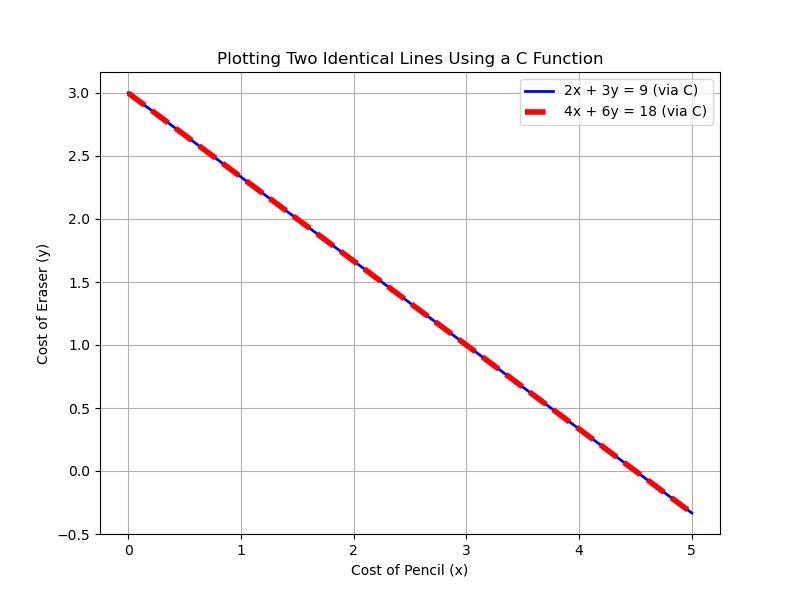
\includegraphics[width = 0.6\columnwidth]{Figure_1.png}
		\caption*{}
		\label{}
	\end{figure}
	\begin{figure}[H]
		\centering
		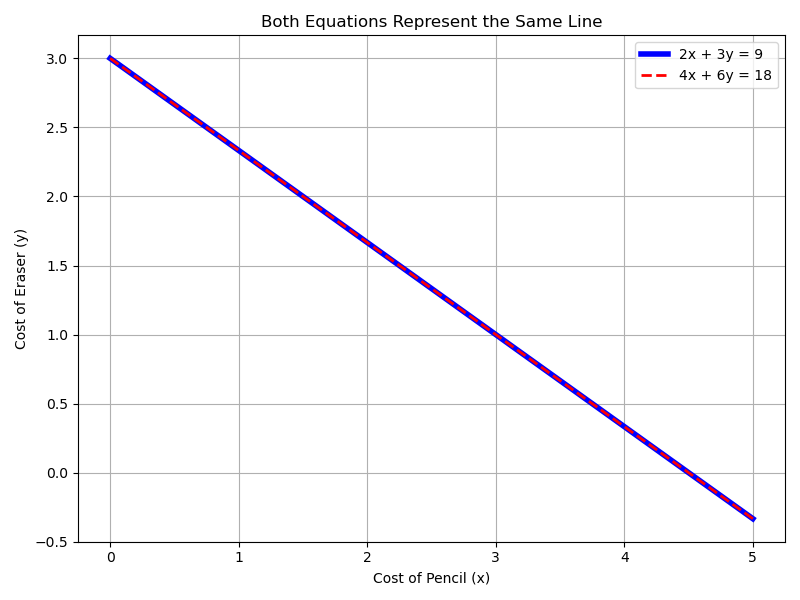
\includegraphics[width = 0.6\columnwidth]{Figure_2.png}
		\caption*{}
		\label{}
	\end{figure}
\end{document}